%%%%%%%%%%%%%%%%%%%%%%%%%%%%
%Capstone Project for Udacity - Juan Jos� Madrigal
%%%%%%%%%%%%%%%%%%%%%%%%%%%%

%%%%%% Packages

\documentclass[11pt]{article}
\usepackage[latin1]{inputenc}
\usepackage{graphicx}
\usepackage{hyperref}
\usepackage[none]{hyphenat}
\hypersetup{colorlinks,urlcolor=light,citecolor=light}
\usepackage{multicol}
\usepackage{array}
\usepackage{cancel}
\usepackage{color}
\usepackage{amssymb}
\usepackage{amsopn}
\usepackage{amsmath}
\usepackage[shortlabels]{enumitem}
\usepackage[default,osfigures,scale=0.95]{opensans}
\setlength{\hoffset}{-1.85cm}
\setlength{\voffset}{-2.5cm}
\setlength{\textwidth}{469pt}
\setlength{\textheight}{640pt}
\setlength{\parindent}{0cm}
\definecolor{dark}{rgb}{0.15,0.30,0.4}
\definecolor{light}{rgb}{0.15,0.3,0.6}

%%%%%% Document

\begin{document}
	
	%%% Header
	
	\begin{center}
		{{\Large\textsc{\color{dark}Machine Learning Engineer Nanodegree}}}\\
		\vspace{0.3cm}
		{{\LARGE\textsc{\color{dark}Capstone Project}}}
	\end{center}
	
	\vspace{-0.4cm}
	
	\textcolor{dark}{\rule{\textwidth}{3pt}}
	
	%%% Personal data
	
	\begin{minipage}[t]{7cm}
		\flushleft
		Juan Jos� Madrigal Mart�nez\\
		February 5, 2017\\
	\end{minipage}
	\hfill
	%%% Contact
	\begin{minipage}[t]{7cm}
		\flushright
		Madrid, Spain\\
		(+0034) 600 86 32 48\\
		juanjomadrigal326@gmail.com\\
		\href{https://es.linkedin.com/in/juan-jose-madrigal}{LinkedIn} \quad
		\href{https://github.com/jxm-math}{GitHub} \quad
		\href{https://www.kaggle.com/jxmmath}{Kaggle} \quad
		\href{https://profiles.udacity.com/u/juanjosmadrigal}{Udacity}
	\end{minipage}\\\\
	
	\vspace{0.3cm}
	
	{{\Large\textsc{\color{dark}I. Definition}}}
	
	\vspace{-0.25cm}
	
	\textcolor{dark}{\rule{\linewidth}{2pt}} \vspace{-0.2cm}
	
	%(approx. 1-2 pages)
	
	{{\large\textbf{\color{dark}Project Overview}}}
	
	\vspace{0.15cm}
	
	This project aims at building a video analysis system for surveillance purposes. It basically finds and indexes the movement events filmed by a fixed camera.\\
	
	Video surveillance has become a major and widely used tool for multiple issues \cite{video_surveillance} and is supported by many companies \cite{video_surveillance_company_1} \cite{video_surveillance_company_2}. But the huge ammount of information which is usually dealt with has led to the need to use Machine Learning techniques to extract patterns, predictions and other refined information. This approach is being implemented \cite{ml_company_1} and there is much work for Machine Learning engineers to do in this field. \\
	
	An efficient implementation of Machine Learning techniques to video surveillance would prevent users from dealing with a sequential (and manual) search through the (perhaps many hours long) video source, which is rather inefficient, boring and error prone, thus providing a major tool for a wide range of purposes.
	
	\begingroup
	\renewcommand{\section}[2]{}%
	\begin{thebibliography}{}
		\bibitem{video_surveillance}
		\href{https://en.wikipedia.org/wiki/Surveillance#Cameras}{Wikipedia - Surveillance / Cameras}
		
		\bibitem{video_surveillance_company_1}
		\href{https://www.videosurveillance.com/}{VideoSurveillance.com}
		
		\bibitem{video_surveillance_company_2}
		\href{http://www.tyco.com/}{Tyco}
		
		\bibitem{ml_company_1}
		\href{http://briefcam.com/}{Briefcam}
		
	\end{thebibliography}
	\endgroup
	
	%In this section, look to provide a high-level overview of the project in layman?s terms. Questions to ask yourself when writing this section:\\
	
	%Has an overview of the project been provided, such as the problem domain, project origin, and related datasets or input data?\\
	%Has enough background information been given so that an uninformed reader would understand the problem domain and following problem statement?\\
	
	{{\large\textbf{\color{dark}Problem Statement}}}
	
	\vspace{0.15cm}
	
	To apply unsupervised Machine Learning clustering algorithms to detect and quantify the movement events filmed by a fixed camera. The algorithms are to be applied to a tridimensional binary array obtained from the original video after some careful video-preprocessing (see below). Further refinements may also be tackled, such as finding time-parametric curves accurately fitting each movement event. \\
	
	%In this section, you will want to clearly define the problem that you are trying to solve, including the strategy (outline of tasks) you will use to achieve the desired solution. You should also thoroughly discuss what the intended solution will be for this problem. Questions to ask yourself when writing this section:\\
	
	%Is the problem statement clearly defined? Will the reader understand what you are expecting to solve?
	%Have you thoroughly discussed how you will attempt to solve the problem?\\
	%Is an anticipated solution clearly defined? Will the reader understand what results you are looking for?\\
	
	{{\large\textbf{\color{dark}Metrics}}}
	
	\vspace{0.15cm}
	
	The direct metric to tune the main parameters of DBScan (\texttt{eps} and \texttt{min\_samples}) will be the Sum of Square Errors according to the expected value of clusters, which is known on beforehand for each of the training videos.\\
	
	Once the algorithm is accurately tuned, the metric(s) used to estimate the quality of our clustering will comprise
	
	\begin{itemize}
		\item Silhouette Coefficient
		\item Calinski-Harabaz Index
	\end{itemize} 
	
	because these do not require knowledge of the ground truth classes.\\
	
	%In this section, you will need to clearly define the metrics or calculations you will use to measure performance of a model or result in your project. These calculations and metrics should be justified based on the characteristics of the problem and problem domain. Questions to ask yourself when writing this section:\\
	
	%Are the metrics you?ve chosen to measure the performance of your models clearly discussed and defined?\\
	%Have you provided reasonable justification for the metrics chosen based on the problem and solution?\\
	
	{{\Large\textsc{\color{dark}II. Analysis}}}
	
	\vspace{-0.25cm}
	
	\textcolor{dark}{\rule{\linewidth}{2pt}} \vspace{-0.2cm}
	
	%(approx. 2-4 pages)
	
	{{\large\textbf{\color{dark}Data Exploration}}}
	
	\vspace{0.15cm}
	
	The datasets and inputs for this project will be obtained after some video preprocessing made on sample videos. The selected videos are located in \href{https://github.com/jxm-math/capstone_project/tree/master/data/unprocessed_videos}{capstone\_project/data/unprocessed\_videos} and they have been downloaded from \href{http://www.viratdata.org/}{VIRAT Video Dataset} \cite{virat}. The video preprocessing is carried out using the free packages \href{http://scikit-image.org/}{SciKitImage} and \href{http://www.scikit-video.org/}{SciKitVideo} and has been generously provided by \href{http://wardenautomation.com/}{WardenAutomation}.\\
	
	The video preprocessing takes as input a \texttt{.avi} $\texttt{M}\times \texttt{N}$ pixels video and a \texttt{.png} $\texttt{M}\times \texttt{N}$ pixels picture (\textit{background}). For each frame in the video, the frame and the background are compared pixel-wise, and the difference is recorded in a $\texttt{M}\times \texttt{N}$ binary array, where $1$ denotes difference (above some threshold) and $0$ denotes no difference.
	
	\begin{center}
		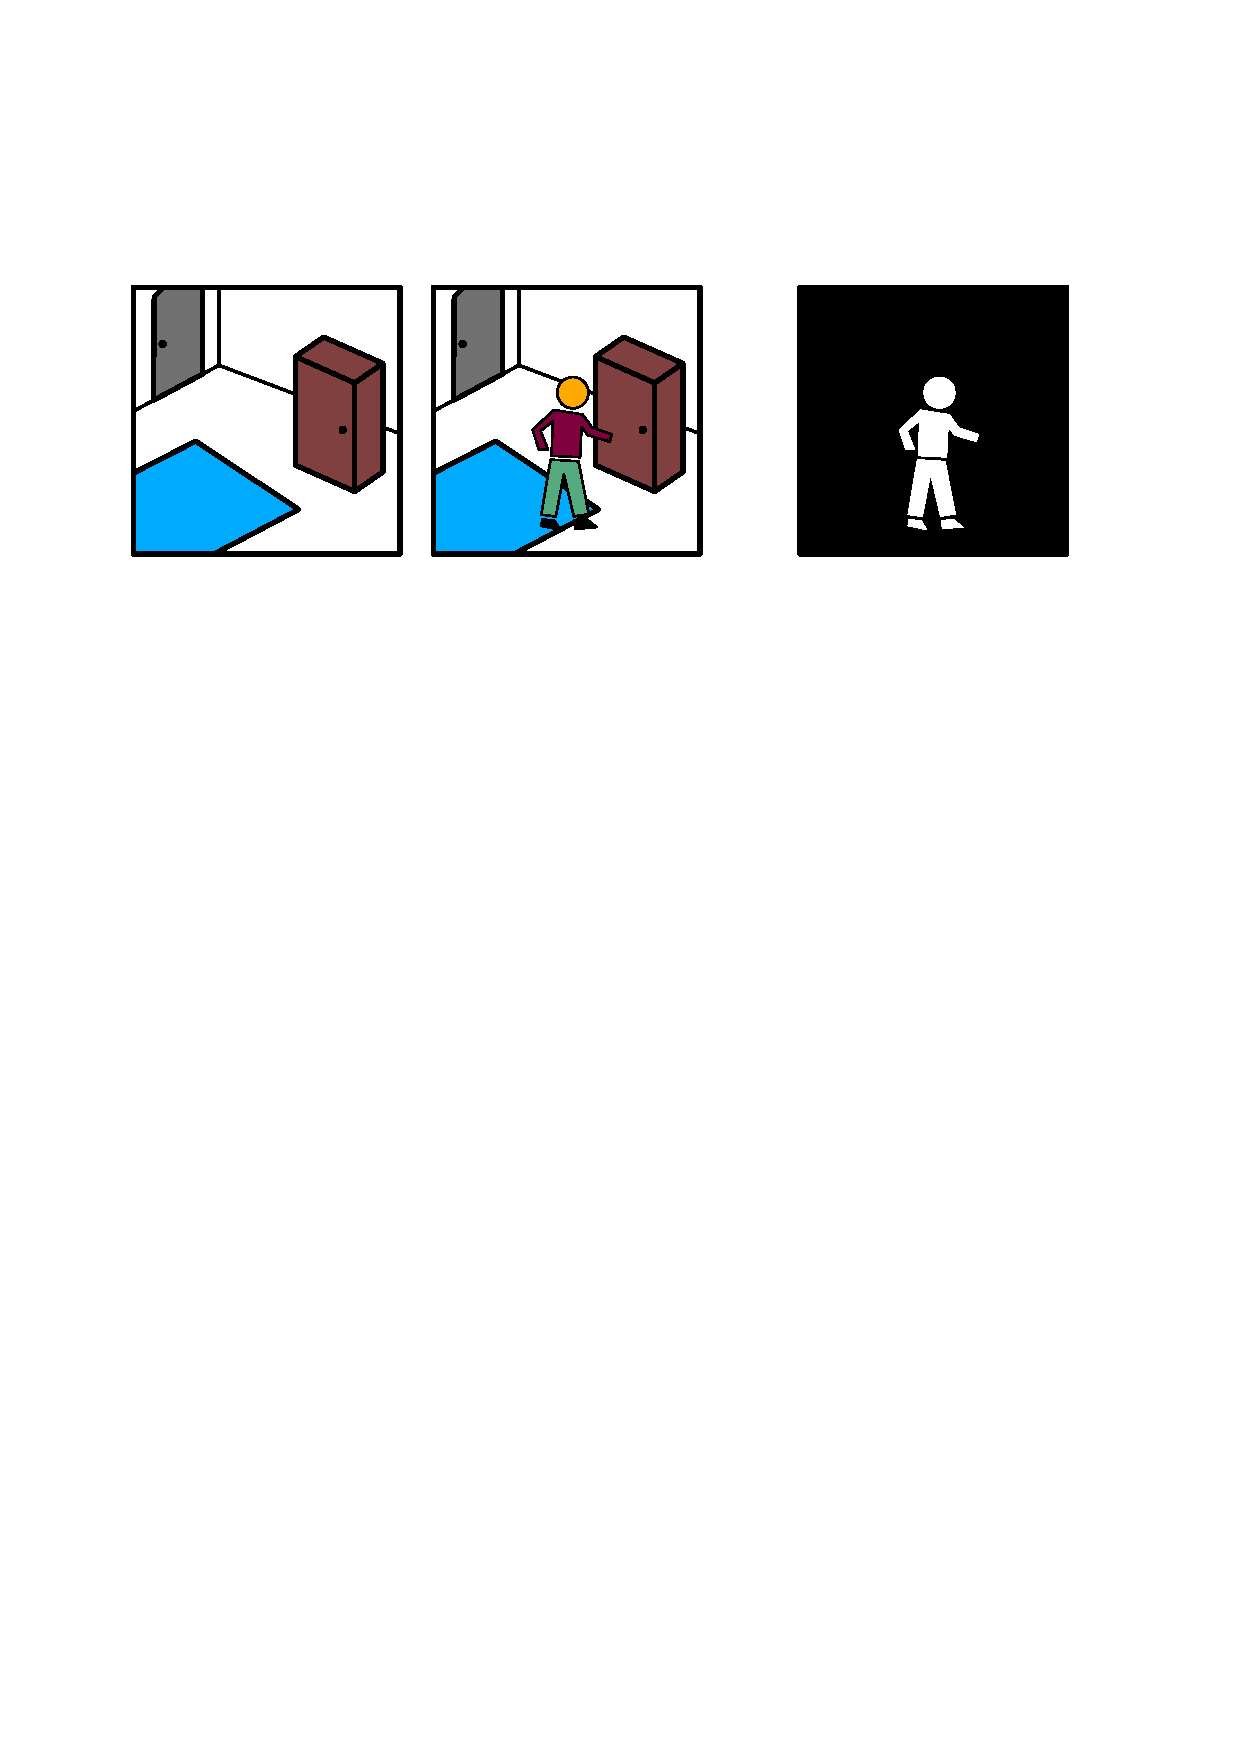
\includegraphics[scale=1]{cpj_1.pdf}
	\end{center}
	
	If the video has $\texttt{T}$ frames, then the video preprocessing gives as output a $\texttt{M}\times \texttt{N}\times \texttt{T}$ binary array, which is supposed to capture the movement in our scene and that will be the primary input for the project. These arrays are saved not as arrays as such but as \texttt{.avi} files, and are located in \href{https://github.com/jxm-math/capstone_project/tree/master/data/processed_videos}{capstone\_project/data/processed\_videos}.\\
	
	\begin{center}
		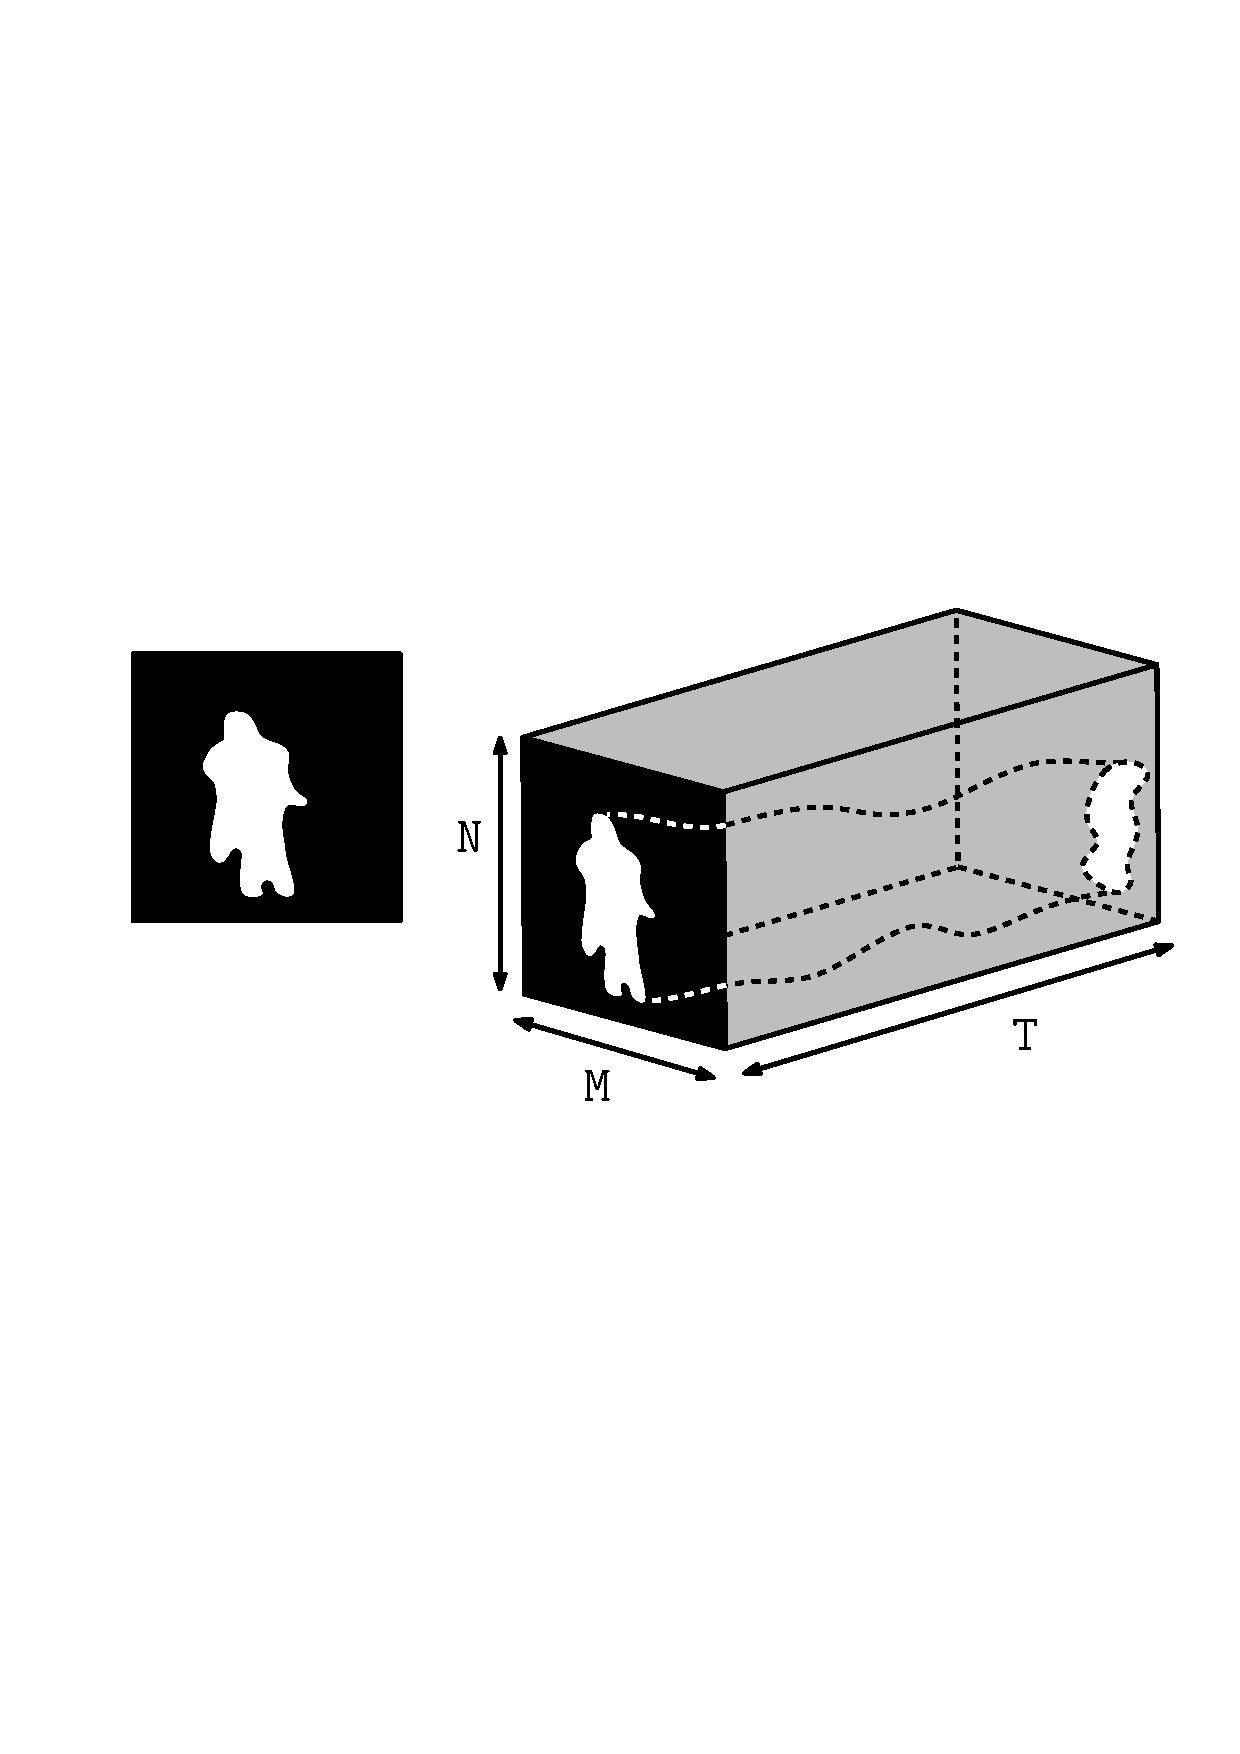
\includegraphics[scale=0.8]{cpj_2.pdf}
	\end{center}
	
	The total ammount of data in this latter folder sums up to 10 videos (and a exploratory \texttt{video1.avi}) whose duration ranges between half and three minutes. This should be enough to tune our algorithm (see below) for the purposes of similar (fixed-camera) videos.
	
	\begingroup
	\renewcommand{\section}[2]{}%
	\begin{thebibliography}{}
		\bibitem{virat}
		\textbf{A Large-scale Benchmark Dataset for Event Recognition in Surveillance Video}, Sangmin Oh, Anthony Hoogs, Amitha Perera, Naresh Cuntoor, Chia-Chih Chen, Jong Taek Lee, Saurajit Mukherjee, J.K. Aggarwal, Hyungtae Lee, Larry Davis, Eran Swears, Xiaoyang Wang, Qiang Ji, Kishore Reddy, Mubarak Shah, Carl Vondrick, Hamed Pirsiavash, Deva Ramanan, Jenny Yuen, Antonio Torralba, Bi Song, Anesco Fong, Amit Roy-Chowdhury, and Mita Desai, \textit{Proceedings of IEEE Comptuer Vision and Pattern Recognition (CVPR), 2011}.
	\end{thebibliography}
	\endgroup
	
	%In this section, you will be expected to analyze the data you are using for the problem. This data can either be in the form of a dataset (or datasets), input data (or input files), or even an environment. The type of data should be thoroughly described and, if possible, have basic statistics and information presented (such as discussion of input features or defining characteristics about the input or environment). Any abnormalities or interesting qualities about the data that may need to be addressed have been identified (such as features that need to be transformed or the possibility of outliers). Questions to ask yourself when writing this section:\\
	
	%If a dataset is present for this problem, have you thoroughly discussed certain features about the dataset? Has a data sample been provided to the reader?\\
	%If a dataset is present for this problem, are statistics about the dataset calculated and reported? Have any relevant results from this calculation been discussed?\\
	%If a dataset is not present for this problem, has discussion been made about the input space or input data for your problem?\\
	%Are there any abnormalities or characteristics about the input space or dataset that need to be addressed? (categorical variables, missing values, outliers, etc.)\\
	
	{{\large\textbf{\color{dark}Exploratory Visualization}}}
	
	\vspace{0.15cm}
	
	The two first \texttt{Jupyter} notebooks deal with some exploratory visualisation\\
	
	\href{https://github.com/jxm-math/capstone_project/blob/master/1.%20data_extractor.ipynb}{\textbf{capstone\_project/1. data\_extractor.ipynb}}\\
	
	Some of the frames of an exploratory video:
	
	\begin{center}
		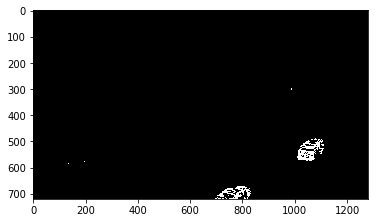
\includegraphics[scale=0.6]{data_exp1.png}
		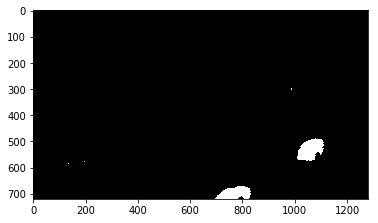
\includegraphics[scale=0.6]{data_exp2.png}
		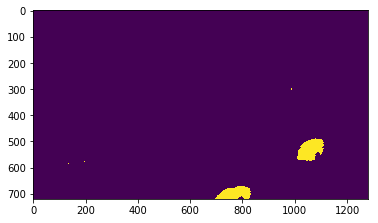
\includegraphics[scale=0.6]{data_exp3.png}
		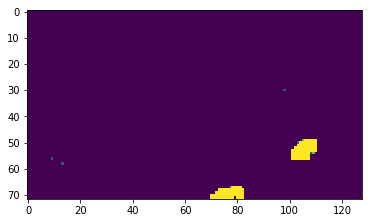
\includegraphics[scale=0.6]{data_exp4.png}
	\end{center}
	
	\begin{enumerate}
		\item Single frame of video
		\item Same frame after applying \texttt{dilation} and \texttt{erosion}
		\item One layer of the previous frame
		\item Dimensionality reduction (\texttt{rescale})
	\end{enumerate}
	
	\href{https://github.com/jxm-math/capstone_project/blob/master/2.%20exploration_clustering.ipynb}{\textbf{capstone\_project/2. exploration\_clustering.ipynb}}\\
	
	Visualisation of point clouds:
	
	\begin{center}
		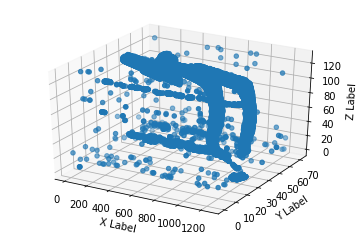
\includegraphics[scale=0.6]{exp_clus1.png}
		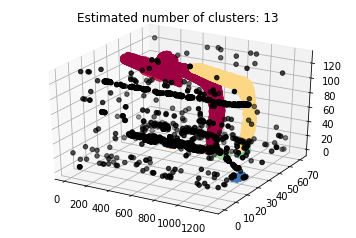
\includegraphics[scale=0.6]{exp_clus2.png}
	\end{center}
	
	\begin{enumerate}
		\item Cloud of points related to an exploratory video
		\item Cloud of points after running \texttt{DSCan} algorithm
	\end{enumerate}
	
	%In this section, you will need to provide some form of visualization that summarizes or extracts a relevant characteristic or feature about the data. The visualization should adequately support the data being used. Discuss why this visualization was chosen and how it is relevant. Questions to ask yourself when writing this section:\\
	
	%Have you visualized a relevant characteristic or feature about the dataset or input data?
	%Is the visualization thoroughly analyzed and discussed?\\
	%If a plot is provided, are the axes, title, and datum clearly defined?\\
	
	{{\large\textbf{\color{dark}Algorithms and Techniques}}}
	
	\vspace{0.15cm}
	
	We propose the use of \href{http://scikit-learn.org/stable/modules/clustering.html#dbscan}{DBSCAN clustering algorithm}, which is implemented in \href{http://scikit-learn.org/}{SciKitLearn}. This clustering algorithm is well-suited for our generic clusters, which are uneven in size and non-convex.\\
	
	DBSCAN clustering algorithm (\textit{Density-based spatial clustering of applications with noise}) takes primarily two parameters
	
	\begin{itemize}
		\item \texttt{min\_samples}, integer
		\item \texttt{eps}, float
	\end{itemize}
	
	and classifies the points in a metric space into three groups
	
	\begin{itemize}
		\item \textbf{Core points}: points whose \texttt{eps}-neighbourhood contains at least \texttt{min\_samples} points
		\item \textbf{Reachable points}: points that are not core points themselves, but that cointain some core point in their \texttt{eps}-neighbourhood
		\item \textbf{Outliers or noise}: points that are not core points nor reachable points
	\end{itemize}
	
	\begin{center}
		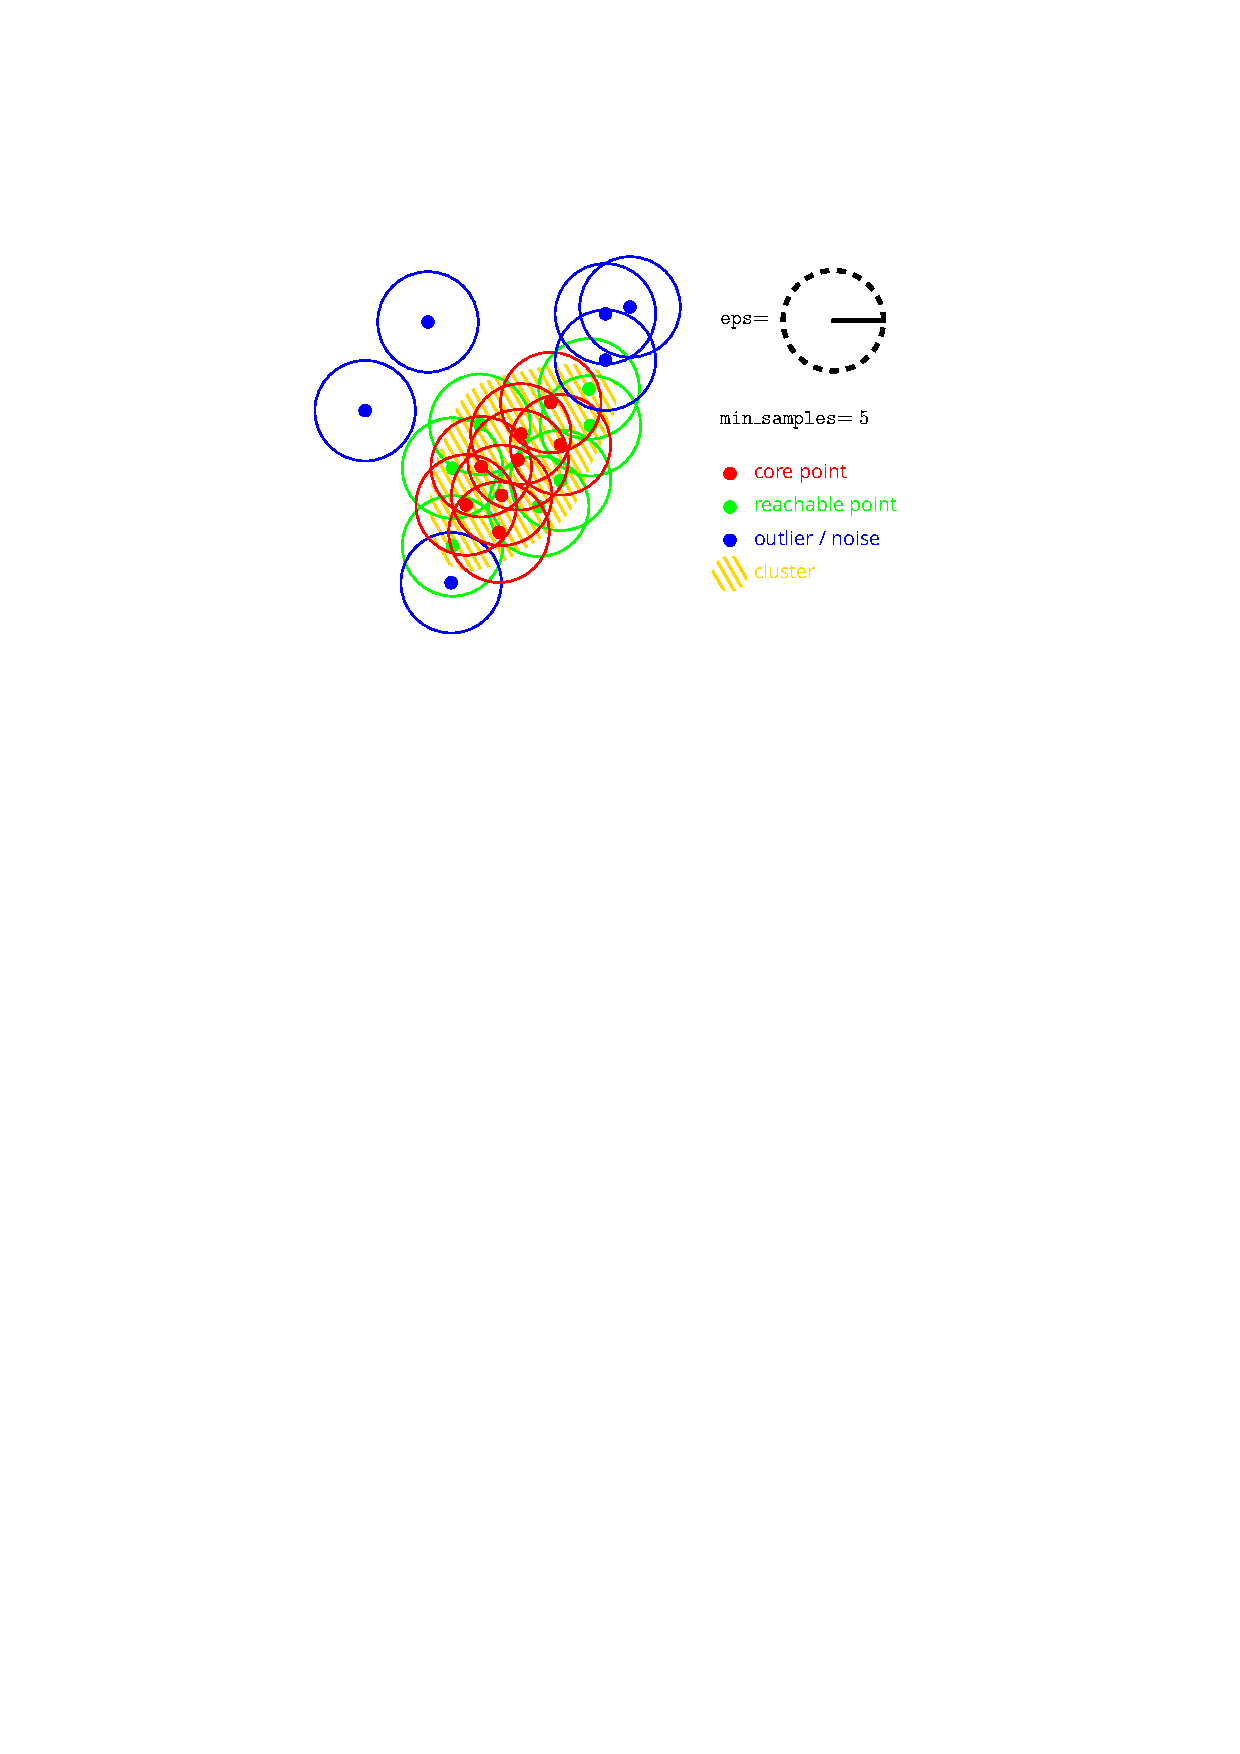
\includegraphics[scale=1.2]{dbscan_illustration.pdf}
	\end{center}
	
	Each group of mutually \texttt{eps}-path-connected core points with the associated reachable points forms a cluster. The way in which the algorithm is implemented may lead to some indeterminisms, such as reachable points reached from two different clusters, but the number of clusters and their intrinsic shape are well-determined.\\
	
	This algorithm has some major advantages that make it well-suited for our clustering problem:
	
	\begin{itemize}
		\item The number of expected clusters is not to be specified. This is crucial, since our goal is to determine the number of clusters / movement-events
		\item The clusters may be of any shape
		\item The algorithm deals well with noise (our arrays, generated from video processing, always have noise)
	\end{itemize} 
	
	\begingroup
	\renewcommand{\section}[2]{}%
	\begin{thebibliography}{}
		\bibitem{dbscan_wikipedia}
		\href{https://en.wikipedia.org/wiki/DBSCAN}{DBScan - Wikipedia}
	\end{thebibliography}
	\endgroup
	
	%In this section, you will need to discuss the algorithms and techniques you intend to use for solving the problem. You should justify the use of each one based on the characteristics of the problem and the problem domain. Questions to ask yourself when writing this section:\\
	
	%Are the algorithms you will use, including any default variables/parameters in the project clearly defined?\\
	%Are the techniques to be used thoroughly discussed and justified?
	%Is it made clear how the input data or datasets will be handled by the algorithms and techniques chosen?\\
	
	{{\large\textbf{\color{dark}Benchmark}}}
	
	\vspace{0.15cm}
	
	A major Benchmark Model may be found at \href{http://www.wisdom.weizmann.ac.il/~vision/VideoAnalysis/Demos/SpaceTimeActions/SpaceTimeActions_pami07.pdf}{Actions as Space-Time Shapes}.\\
	
	This work deals with the recognition of activities in a single movement-event. For this movement-event to be analysed, spectral clustering methods are used \cite{spectral_clustering_wikipedia}. The performance is measured in terms of misclassifications (2.17\%, 7.91\% and 36.40\% for different methods). 
	
	\begingroup
	\renewcommand{\section}[2]{}%
	\begin{thebibliography}{}
		\bibitem{spectral_clustering_wikipedia}
		\href{https://en.wikipedia.org/wiki/Spectral_clustering}{Spectral Clustering - Wikipedia}
	\end{thebibliography}
	\endgroup
	
	%In this section, you will need to provide a clearly defined benchmark result or threshold for comparing across performances obtained by your solution. The reasoning behind the benchmark (in the case where it is not an established result) should be discussed. Questions to ask yourself when writing this section:\\
	
	%Has some result or value been provided that acts as a benchmark for measuring performance?\\
	%Is it clear how this result or value was obtained (whether by data or by hypothesis)?\\
	
	{{\Large\textsc{\color{dark}III. Methodology}}}
	
	\vspace{-0.25cm}
	
	\textcolor{dark}{\rule{\linewidth}{2pt}} \vspace{-0.2cm}
	
	%(approx. 3-5 pages)
	
	{{\large\textbf{\color{dark}Data Preprocessing}}}
	
	\vspace{0.15cm}
	
	The first step in the data preprocessing has been generously provided by \href{http://wardenautomation.com/}{WardenAutomation}. It consists in the extraction of \textit{movement masks}, with the method described above, processing the videos in \href{https://github.com/jxm-math/capstone_project/tree/master/data/unprocessed_videos}{unprocessed\_videos} into those of \href{https://github.com/jxm-math/capstone_project/tree/master/data/processed_videos}{processed\_videos}.\\
	
	The second step in the data preprocessing is carried out by the \texttt{Jupyter} notebook \href{https://github.com/jxm-math/capstone_project/blob/master/data_extractor.ipynb}{data\_extractor.ipynb}. For each frame in the movement masks, it applies
	
	\begin{enumerate}[a)]
		\item Several \texttt{dilation} and \texttt{erosion} processes
		\item Extraction of one color layer
		\item Dimensionality reduction (\texttt{rescale})
	\end{enumerate}
	
	and finally stores the coordinates of the movement points in \texttt{NumPy} arrays in the folder \href{https://github.com/jxm-math/capstone_project/tree/master/data/numpy_arrays}{numpy\_arrays}.\\
	
	%In this section, all of your preprocessing steps will need to be clearly documented, if any were necessary. From the previous section, any of the abnormalities or characteristics that you identified about the dataset will be addressed and corrected here. Questions to ask yourself when writing this section:\\
	
	%If the algorithms chosen require preprocessing steps like feature selection or feature transformations, have they been properly documented?\\
	%Based on the Data Exploration section, if there were abnormalities or characteristics that needed to be addressed, have they been properly corrected?\\
	%If no preprocessing is needed, has it been made clear why?\\
	
	{{\large\textbf{\color{dark}Implementation}}}
	
	\vspace{0.15cm}
	
	The implementation of the \texttt{DBScan} algorithm is remarkably easy:\\
	
	\begin{quote}
	\begin{verbatim}
	db = DBSCAN(eps=3, min_samples=20).fit(data)
	labels = db.labels_
	
	# Number of clusters in labels, ignoring noise if present.
	n_clusters_ = len(set(labels)) - (1 if -1 in labels else 0)
	
	print('Estimated number of clusters: %d' % n_clusters_)
	\end{verbatim}
	\end{quote}
	
	where \texttt{data} is the arrays of points to be clustered.\\
	
	%In this section, the process for which metrics, algorithms, and techniques that you implemented for the given data will need to be clearly documented. It should be abundantly clear how the implementation was carried out, and discussion should be made regarding any complications that occurred during this process. Questions to ask yourself when writing this section:\\
	
	%Is it made clear how the algorithms and techniques were implemented with the given datasets or input data?\\
	%Were there any complications with the original metrics or techniques that required changing prior to acquiring a solution?\\
	%Was there any part of the coding process (e.g., writing complicated functions) that should be documented?\\
	
	{{\large\textbf{\color{dark}Refinement}}}
	
	\vspace{0.15cm}
	
	The notebook \href{https://github.com/jxm-math/capstone_project/blob/master/3.%20parameter_tuning.ipynb}{3. parameter\_tuning.ipynb} deals with the identification of the optimal parameters \texttt{eps} and \texttt{min\_samples} inside the \texttt{DBScan} algorithm. For each of the exploratory pairs
	
	\begin{quote}
		\begin{verbatim}
		eps in [2,4,6,8,10,12,14,16,18,20]
		min_samples in [40,80,120,160,200,240,280,320,360,400,
		    440,480,520,560,600,640,680,720,760,800]
		\end{verbatim}
	\end{quote}
	
	a \texttt{DBScan} method has been applied to the training data and a Sum of Square Errors (when comparing the output with the expected output registered by direct observation of the original videos) has been stored. The pair in which the best local minimal has been achieved is \texttt{eps = 6 , min\_samples = 400}, and this values have been used for the final implementation.\\
	
	%In this section, you will need to discuss the process of improvement you made upon the algorithms and techniques you used in your implementation. For example, adjusting parameters for certain models to acquire improved solutions would fall under the refinement category. Your initial and final solutions should be reported, as well as any significant intermediate results as necessary. Questions to ask yourself when writing this section:\\
	
	%Has an initial solution been found and clearly reported?\\
	%Is the process of improvement clearly documented, such as what techniques were used?\\
	%Are intermediate and final solutions clearly reported as the process is improved?\\
	
	{{\Large\textsc{\color{dark}IV. Results}}}
	
	\vspace{-0.25cm}
	
	\textcolor{dark}{\rule{\linewidth}{2pt}} \vspace{-0.2cm}
	
	%(approx. 2-3 pages)
	
	{{\large\textbf{\color{dark}Model Evaluation and Validation}}}
	
	\vspace{0.15cm}
	
	The notebook \href{https://github.com/jxm-math/capstone_project/blob/master/4.%20implementation_validation.ipynb}{4. implementation\_validation.ipynb} deals with the evaluation and validation.\\
		
	Our tuned \texttt{DBScan} algorithm is applied to our training videos. We compare the expected clusters and the output given. We also measure the Silhouette Coefficient \cite{silhouette_coefficient} and the Calinski-Harabaz Index \cite{calinski_harabaz_index}. Some of the calculations give rise to a \texttt{Memory Error}, so we do not have the scores for every training video.\\
	
	\begingroup
	\renewcommand{\section}[2]{}%
	\begin{thebibliography}{}
		\bibitem{silhouette_coefficient}
		\href{http://scikit-learn.org/stable/modules/clustering.html#silhouette-coefficient}{Silhouette Coefficient - SKLearn}
		\bibitem{calinski_harabaz_index}
		\href{http://scikit-learn.org/stable/modules/clustering.html#calinski-harabaz-index}{Calinski-Harabaz Index - SKLearn}
	\end{thebibliography}
	\endgroup

	
	%In this section, the final model and any supporting qualities should be evaluated in detail. It should be clear how the final model was derived and why this model was chosen. In addition, some type of analysis should be used to validate the robustness of this model and its solution, such as manipulating the input data or environment to see how the model?s solution is affected (this is called sensitivity analysis). Questions to ask yourself when writing this section:\\
	
	%Is the final model reasonable and aligning with solution expectations? Are the final parameters of the model appropriate?\\
	%Has the final model been tested with various inputs to evaluate whether the model generalizes well to unseen data?\\
	%Is the model robust enough for the problem? Do small perturbations (changes) in training data or the input space greatly affect the results?\\
	%Can results found from the model be trusted?\\
	
	{{\large\textbf{\color{dark}Justification}}}
	
	\vspace{0.15cm}
	
	The results obtained (\href{https://github.com/jxm-math/capstone_project/blob/master/4.%20implementation_validation.ipynb}{4. implementation\_validation.ipynb}) are quite good, but not excellent; further improvement should be done.\\
		
	Comparing our results with those in our Benchmark Model \href{http://www.wisdom.weizmann.ac.il/~vision/VideoAnalysis/Demos/SpaceTimeActions/SpaceTimeActions_pami07.pdf}{Actions as Space-Time Shapes}, we may appreciate that the last ones also run into a great number of misclassifications (2.17\%, 7.91\% and 36.40\% for different methods). This shows that the movement-events recognition is in general quite a difficult problems where major Machine Learning techniques have to be studied and implemented.\\ 
	
	%In this section, your model?s final solution and its results should be compared to the benchmark you established earlier in the project using some type of statistical analysis. You should also justify whether these results and the solution are significant enough to have solved the problem posed in the project. Questions to ask yourself when writing this section:\\
	
	%Are the final results found stronger than the benchmark result reported earlier?\\
	%Have you thoroughly analyzed and discussed the final solution?\\
	%Is the final solution significant enough to have solved the problem?\\
	
	{{\Large\textsc{\color{dark}V. Conclusion}}}
	
	\vspace{-0.25cm}
	
	\textcolor{dark}{\rule{\linewidth}{2pt}} \vspace{-0.2cm}
	
	%(approx. 1-2 pages)
	
	{{\large\textbf{\color{dark}Free-Form Visualization}}}
	
	\vspace{0.15cm}
	
	The notebook \href{https://github.com/jxm-math/capstone_project/blob/master/5.%20final_visualisation.ipynb}{5. final\_visualisation.ipynb} deals with the final visualisation.\\
		
	\begin{center}
		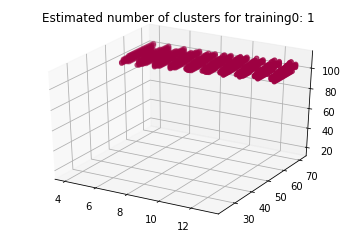
\includegraphics[scale=0.6]{vis0.png}
		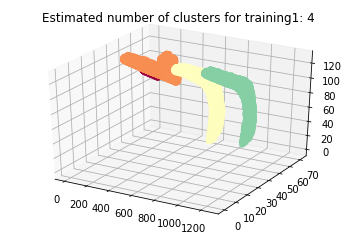
\includegraphics[scale=0.6]{vis1.png}
		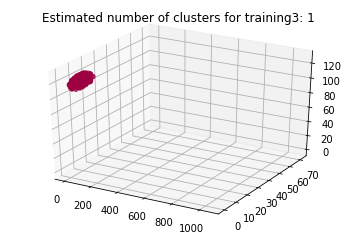
\includegraphics[scale=0.6]{vis3.png}
		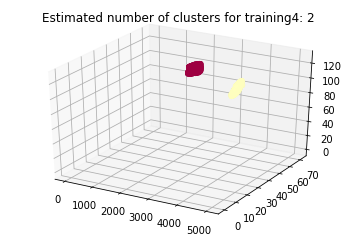
\includegraphics[scale=0.6]{vis4.png}
		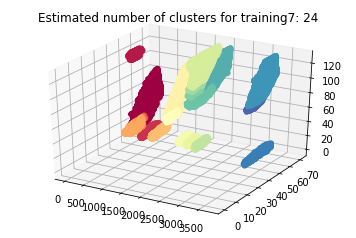
\includegraphics[scale=0.6]{vis7.png}
		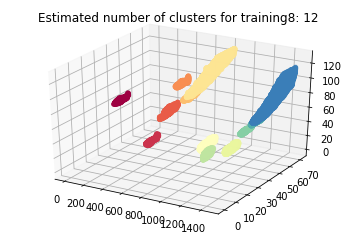
\includegraphics[scale=0.6]{vis8.png}
	\end{center}
	
	%In this section, you will need to provide some form of visualization that emphasizes an important quality about the project. It is much more free-form, but should reasonably support a significant result or characteristic about the problem that you want to discuss. Questions to ask yourself when writing this section:\\
	
	%Have you visualized a relevant or important quality about the problem, dataset, input data, or results?\\
	%Is the visualization thoroughly analyzed and discussed?\\
	%If a plot is provided, are the axes, title, and datum clearly defined?\\
	
	{{\large\textbf{\color{dark}Reflection}}}
	
	\vspace{0.15cm}
	
	This Udacity ML Nanodegree Capstone Project has been a very enriching experience. It has been difficult but it has provided most encouraging results.\\
	
	Perhaps the toughest part in the project has been the video preprocessing. It needed a lot of memory and time, so several methods had to be implemented (e.g. the use of Python generators instead of list comprehension) until finding one that could properly deal with such huge datasets.\\
	
	The posterior tuning and validation has also been quite a subtle point. Almost all the clustering metrics assume knowledge of the ground truth classes, which in our setting is totally non-viable (even when the movement-events may be enumerated by direct visualisation).\\
	
	%In this section, you will summarize the entire end-to-end problem solution and discuss one or two particular aspects of the project you found interesting or difficult. You are expected to reflect on the project as a whole to show that you have a firm understanding of the entire process employed in your work. Questions to ask yourself when writing this section:\\
	
	%Have you thoroughly summarized the entire process you used for this project?\\
	%Were there any interesting aspects of the project?\\
	%Were there any difficult aspects of the project?\\
	%Does the final model and solution fit your expectations for the problem, and should it be used in a general setting to solve these types of problems?\\
	
	{{\large\textbf{\color{dark}Improvement}}}
	
	\vspace{0.15cm}
	
	There are several aspects in which this method may be improved in further work:
	
	\begin{itemize}
		\item The movement masks extraction algorithm may be tuned to capture better the movement-events.
		\item The \texttt{eps} and \texttt{min\_samples} parameters could be dynamically tuned in function of the input, if different fixed-camera contexts are to be considered. For instance, different parameters would be needed for driving cars or walking people. 
	\end{itemize} 
	
	%In this section, you will need to provide discussion as to how one aspect of the implementation you designed could be improved. As an example, consider ways your implementation can be made more general, and what would need to be modified. You do not need to make this improvement, but the potential solutions resulting from these changes are considered and compared/contrasted to your current solution. Questions to ask yourself when writing this section:\\
	
	%Are there further improvements that could be made on the algorithms or techniques you used in this project?
	%Were there algorithms or techniques you researched that you did not know how to implement, but would consider using if you knew how?
	%If you used your final solution as the new benchmark, do you think an even better solution exists?\\


%Before submitting, ask yourself. . .

%Does the project report you?ve written follow a well-organized structure similar to that of the project template?

%Is each section (particularly Analysis and Methodology) written in a clear, concise and specific fashion? Are there any ambiguous terms or phrases that need clarification?

%Would the intended audience of your project be able to understand your analysis, methods, and results?

%Have you properly proof-read your project report to assure there are minimal grammatical and spelling mistakes?

%Are all the resources used for this project correctly cited and referenced?

%Is the code that implements your solution easily readable and properly commented?

%Does the code execute without error and produce results similar to those reported?

\end{document}
